\documentclass[main.tex]{subfiles}
\begin{document}
\onlyinsubfile{\mainmatter{}}

\chapter{Background: Ensuring Memory Safety using Capabilities}
Most security bugs classified as \enquote{serious} in large projects such as the Chromium browser engine are memory safety bugs,\cite{chromium} such as out-of-bounds array or call stack accesses that either arise from the use of \enquote{memory-unsafe} programming languages such as C, the use of memory safety opt-outs (such as Rust’s \texttt{unsafe}) in \enquote{memory-safe} programming languages, or bugs in the compiler or standard library implementation of a memory-safe programming language or runtime environment such as the Java VM or an ECMAScript interpreter.

Common approaches to mitigating attacks or restricting the attack vector that such a bug can cause include reintroducing compiler-inserted array bounds checks in memory-unsafe programming languages and enforcing page-level permissions in the virtual memory system of the operating system. However, runtime checks introduce a runtime cost, and virtual memory protection doesn’t protect against a compromised or vulnerable library such as Apache Log4j accessing potentially sensitive data in the process’ address space such as TLS session keys stored in an in-process OpenSSL data structure.

A different approach are capabilities, which are usually unforgeable pointers that carry authority over a precise region of memory and with a precise set of permissions, thereby providing fine-grained memory protection. To ensure that authority cannot be created, capabilities can only be derived from a source with more authority, such as an operating system, a more privileged routine, or another capability. Finally, capability support can be provided at the hardware level, removing the runtime cost associated with software-based bounds \& permission checks.

\section{Capability Hardware Enhanced RISC Instructions}
CHERI (Capability Hardware Enhanced RISC Instructions; see also \cite{intro2cheri}) is a design for a capability machine, extending several existing instruction set architectures (ISAs) such as RISC-V, MIPS, x86-64, and Arm with hardware capability support. One of CHERI’s design goals is to provide a viable transition path for mainstream systems. An ecosystem formed around CHERI, such as capability extensions for C \& C++, capability support in the LLVM compiler toolchain and QEMU emulator, a FreeBSD fork with capability support called CheriBSD, and several large libraries and systems such as PostgreSQL and WebKit being ported to CheriBSD.

In 64-bit CHERI-RISC-V, the CHERI extension of the 64-bit RISC-V ISA, 64-bit pointers become 128-bit capabilities. As illustrated in \cref{fig:chericoncentrate}, such a capability consists of a 64-bit address, a 27-bit compressed value indicating the capability’s bounds, a 16-bit permissions mask (specifying permissions such as \emph{permit load}), with the remaining 21 bits reserved for encoding other flags and the capability’s object type (used for a CHERI feature called \enquote{sealing}, cf. infra). A 1-bit validity tag stored out-of-band in tagged memory is set when the 128-bit datum represents a valid capability, and cleared whenever the datum is modified by any instruction not intended to validly modify capabilities (such as \texttt{XOR} or \texttt{ADD}).

CHERI-RISC-V defines several capability-aware instructions that can validly modify capability within specified constraints. For instance, \texttt{CAndPerm} removes permissions from a given capability by performing a bitwise conjunction with a given permissions mask whereas \texttt{CIncOffset} adds an offset to a given capability's address. These limitations are in place to ensure 4 important safety properties of capability machines and CHERI architectures in particular, briefly summarised here below.

\begin{figure}
	\begin{center}
		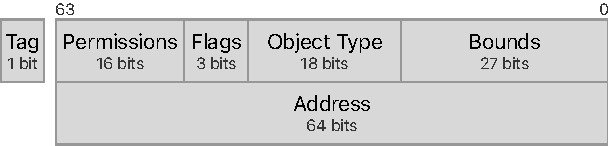
\includegraphics{Images/CHERI Concentrate Layout.pdf}
	\end{center}
	\caption{A simplified layout of a 256-bit CHERI capability compressed into 128 bits using the CHERI Concentrate encoding. CHERI-RISC-V defines one flag bit and reserves the other two bits for future use. The validity tag bit is stored out-of-band, usually in tagged memory not directly accessible by user programs.}
	\label{fig:chericoncentrate}
\end{figure}

\paragraph{Permissions} A capability specifies zero or more permissions that the holder of the capability is allowed to do using that capability. For example, the \emph{permit load} resp. \emph{permit store} permissions allow the holder to load resp. store data in the region of memory specified by the capability. Beyond permissions also found in traditional virtual memory systems, capabilities also support CHERI-specific permissions such as \emph{allow local capability store} and \emph{permit seal}. Performing an action not allowed by the capability, such as storing data using a load-only capability, results in a machine trap.\footnote{In some specific cases, such as loading a capability using a capability that only allows loading data but not capabilities, merely results in a capability's tag being cleared, thereby deactivating any authority that it otherwise might've unintentionally conferred.}

\paragraph{Bounds} A capability specifies a contiguous region of memory where the holder of the capability is allowed exercise actions permitted by the capability's permissions. For example, a capability produced by a secure, capability-aware implementation of \texttt{malloc} pointing to a heap-allocated buffer would only permit accesses within that buffer. Performing an action outside of these bounds, such as a buffer overflow, results in a machine trap.

\paragraph{Provenance} A capability can only be derived from other capabilities. Authority cannot be forged by modifying its in-memory representation; attempting to do so causes the capability's tag bit to be cleared which invalidates the capability. Tag bits cannot be set in software.

\paragraph{Monotonicity} A capability cannot have more authority than the capability it's derived from: permissions can only be removed and bounds can only be shrunk. At CPU reset, the hardware provides root capabilities to the bootloader or firmware, which can be iteratively restricted in higher levels of abstraction, as illustrated in \cref{fig:derivingauth}.

\begin{figure}
	\begin{center}
		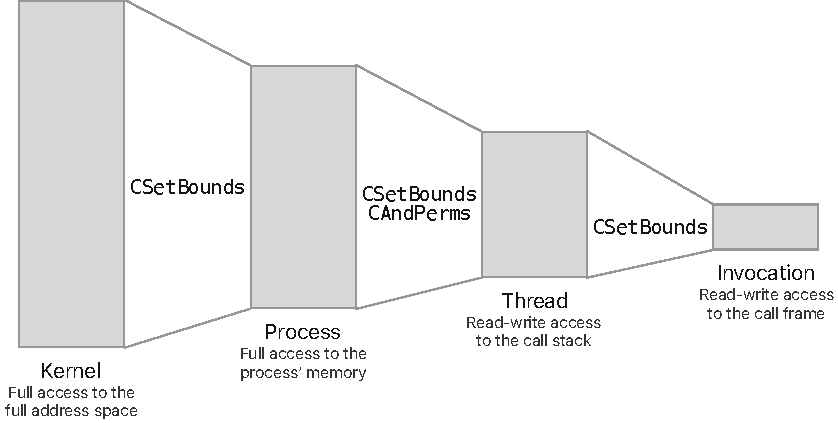
\includegraphics{Images/Deriving Authority.pdf}
	\end{center}
	\caption{Provenance and monotonicity in action in protecting process memory, the call stack, and a call frame. The size of the depicted memory regions are not to scale. Similar illustrations can be made about a process' heap and heap-allocated memory.}
	\label{fig:derivingauth}
\end{figure}

\section{Sealed Capabilities}
CHERI provides a capability protection mechanism called \emph{sealing}, whereby the capability holder is restricted from modifying or dereferencing the capability. The inverse operation, i.e., \emph{unsealing}, is only allowed under specific circumstances. Sealing comes in two forms: sealing using a \emph{seal capability} or sealing as a \emph{sentry (sealed entry) capability}. The sealed state of a capability is encoded in its \emph{object type} field; the object type of an unsealed capability has the special value $-1$.

\paragraph{Sealing using a seal capability} A capability with the \emph{permit seal} permission (the \emph{seal capability}) can be used to seal another capability (the \emph{sealed capability}). The object type of the sealed capability is set to the seal capability's \enquote{address}.\footnote{Note that this \enquote{address} doesn't necessarily need to refer to a valid location in memory. A capability whose address is only used for sealing and unsealing capabilities should therefore omit the \emph{Permit load} and \emph{Permit store} family of permissions.} A capability with the \emph{permit unseal} permission (the \emph{unseal capability}) can be used to unseal a sealed capability provided that the sealed capability's object type matches the unseal capability's \enquote{address} exactly. A seal capability can also act as an unseal capability if it has both permissions.

As would be expected from normal pointer-like capabilities, the (un)seal capability's address must be within its bounds when (un)sealing; otherwise a machine trap ensues. By carefully controlling access to and bounding capabilities with the \emph{permit seal} and \emph{permit unseal} permissions, sealing can be used for higher-level features such as encapsulation.

Sealing and unsealing can be done using the \texttt{CSeal} respectively \texttt{CUnseal} instructions. CHERI-RISC-V additionally provides a \texttt{CInvoke} instruction that takes a code and data capability pair with matching object type, unseals them, and jumps to the code capability's address. This feature enables secure domain transitions, wherein the caller cannot dereference the code or data capability (which may belong to a closure, for example), but can use them to perform an invocation.

\paragraph{Sealing as a sentry capability} An executable capability can be sealed by itself as a sentry capability using the \texttt{CSealEntry} instruction. CHERI-RISC-V defines a \texttt{CJALR} instruction that jumps to the address of a given target capability, unsealing the capability if it is a sentry capability. Similar to RISC-V's \texttt{JALR} instruction, the instruction also accepts a link register wherein it puts the return address. Unlike \texttt{JALR}, \texttt{CJALR} also seals the return capability as a sentry capability, ensuring that the callee can only use it to return to the caller. A sentry capability's object type has the special value $-2$.

\section{Local State Encapsulation \& Well-Bracketed Control Flow}
Capabilities are CHERI’s building blocks on which security features can be built, akin to how cryptographic primitives form the basis of cryptographic algorithms. One low-level application of capabilities is in (1) protecting a component's local state, the so-called local state encapsulation property, and (2) enforcing the return-to-caller principle, a property named well-bracketed control flow.

To illustrate the need for these two properties, let’s look at an example. Suppose Apache httpd invokes a decompression routine in libZIP, however due to a vulnerability in the libZIP routine, an attacker is able to perform a remote code execution using a maliciously crafted ZIP archive. Even if the stack capability —which replaces the stack pointer in conventional systems— is appropriately bounded to the region of memory associated with the current thread’s call stack and the called libZIP routine has no other capabilities into httpd’s data structures, the stack capability still grants the libZIP procedure (and hence the attacker) access to httpd’s stack frames and thus httpd’s local state which, of course, may include sensitive information. Alternatively, the attacker could deviate from the normal calling convention, skip the caller, and return to a caller higher up in the call stack. In order to mitigate these kinds of attacks, several “secure” calling conventions have been proposed in the literature.

One such convention, implemented by CheriBSD, consists of splitting each thread’s call stack into multiple stacks: one stack per component where all stack frames belonging to the component are stored, as well as one trusted stack in kernel memory tying all stack frames together. Each component is in its own compartmentalised security domain, and the stack capability in each component only grants access to that component’s stack memory. An attacker relying on a vulnerable component can no longer access another component’s local state this way and cannot return to an arbitrary caller. However, since it’s the kernel that manages the central cross-component stack, a system call is required to cross a security domain, i.e., to invoke a procedure in a different component.

An alternative calling convention proposed by \cite{retptr} avoids the need for multiple stacks and for syscalls when crossing a security domain by keeping all stack frames in a single call stack and by restricting the stack capability just before the invocation to exclude the region of stack memory containing existing stack frames. Due to the monotonicity property of capabilities, the callee cannot increase the stack capability’s authority to include the excluded region. This safety property however makes it impossible to return to the caller. For this reason, just before jumping to the callee, the caller pushes a special restoration routine onto the stack which includes the previous stack capability as its payload and whose code restores the stack capability. The callee is then provided with a return capability pointing to this routine and bounded to that routine’s memory space; the callee can return to the caller by jumping to the routine. Finally, to thwart attempts by the callee to use this return capability to read the previous stack capability, the return capability is sealed so that it can only be used to invoke the routine and not to read the routine’s code or payload.

This alternative approach as described above is alas not enough to ensure local state encapsulation and well-bracketed control flow if a compromised routine is invoked more than once. An attacker could store its stack capability somewhere during a first invocation and use that capability in a subsequent invocation. If the call stack grows by the time the attacker’s code gets to run again, the previously stored stack capability gives them authority over a larger portion of the stack than the stack capability they get in the second invocation, and thus get access to stack frames from other components.

A first solution is to prohibit writing the stack capability anywhere but on the stack itself, using a CHERI feature called local capabilities, and clearing the unused portion of the stack when returning from a procedure in a different security domain.

Clearing a region of memory is a potentially expensive operation so a second solution by \cite{uninitcaps} is to use a proposed CHERI feature called uninitialised capabilities which forces uninitialised memory regions to be overwritten before they can be read. In this solution, the stack capability is still a local capability as in the first solution, but the unused portion of the stack is marked as uninitialised in the stack capability, avoiding the need for clearing memory.

\biblio{}
\onlyinsubfile{\glsaddall\printglossaries}
\end{document}